\documentclass[accentcolor=tud1b,colorbacktitle,inverttitle,landscape,german,
presentation]{tudbeamer}
\usepackage{graphicx} 
\usepackage{ngerman}
\usepackage[utf8]{inputenc}
\usepackage{booktabs}
\usepackage{wrapfig}
%\usepackage{caption}
%\usepackage{subcaption}
\usepackage{listings}
\renewcommand{\arraystretch}{1.2}
\usepackage{url}
\usepackage{tikz}
\usepackage{multimedia}
%\usepackage{movie9}


%\hypersetup{ colorlinks, citecolor=green, filecolor=black, linkcolor=blue, urlcolor=blue } 

\setbeamertemplate{section in toc}[square]
\setbeamertemplate{subsection in toc}[square]
\setbeamertemplate{bibliography item}{\insertbiblabel}
% \setbeamercolor{example text}{fg=green!50!black}
% \setbeamercolor{block alerted  item}{fg=red}

\setbeamercolor{block title alerted}{fg=red}
%body
%\setbeamercolor{block body alerted}{fg=black!90,bg=brown!60!yellow}
% parent of all alerts default is red
\setbeamercolor{alerted text}{fg=red}

%\setbeamertemplate{caption}{\raggedright\insertcaption\par}


%Activate captions
\setbeamertemplate{caption}{\color{tudtextaccent} Abb.: \color{black}\insertcaption} 


%\graphicspath{{bilder/}}
\begin{document}
  
  \title[]{Entwicklung eines Sensorfusions-Frameworks zur Umgebungsmodellierung}
  \subtitle{Zwischenvortrag Bachelorthesis\\
  Marius Schnaubelt}
  
  \author[M. Schnaubelt]{Marius Schnaubelt}
  \institute[SIM TU Darmstadt]{Fachgebiet Simulation, Systemoptimierung und Robotik, TU Darmstadt}
  
  % \logo{\color{tudtextaccent}\large IFP}
  
  \date{\today}
  
  \begin{titleframe}
    \begin{figure}[htbp] 
      \centering
      
      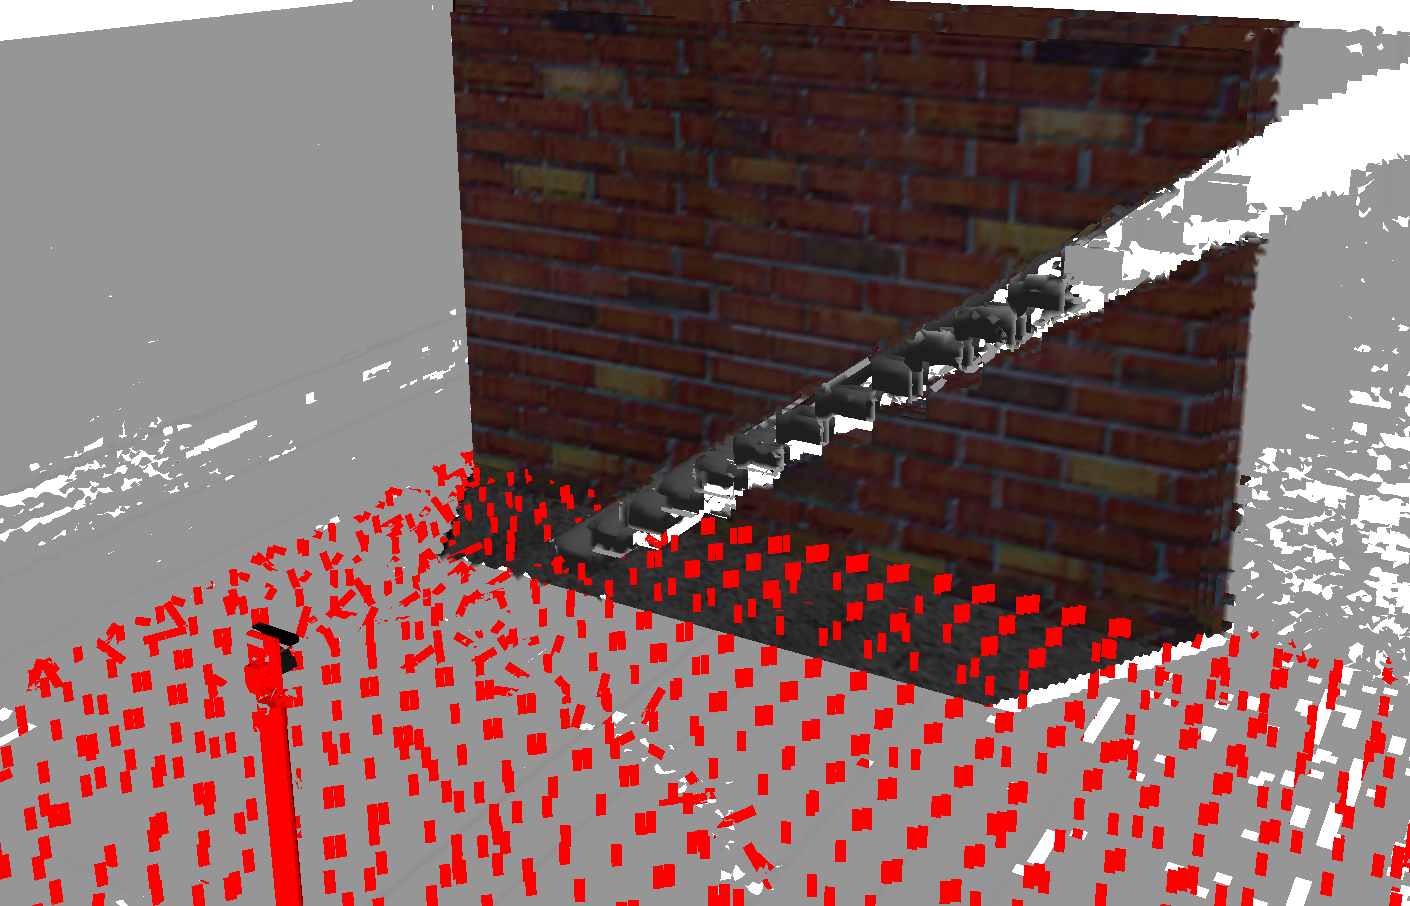
\includegraphics[height=0.45\textwidth]{images/mason_trim} 
      
    \end{figure}
  \end{titleframe}
  
  \section*{Inhalte}
  
  \begin{frame}
    \frametitle{Inhalte}
    \small{\tableofcontents}
  \end{frame}
  
  
  \section{Einleitung}

\begin{frame}[t]
    \frametitle{Einleitung}
    
      \begin{columns}[t]
      \column[]{7cm}
      
      \begin{itemize}
      \item Mobile Roboter besitzen unterschiedliche Sensorsysteme
%       \begin{itemize}
%        \item RGB-Kameras
%        \item RGB-D-Kameras
%        \item Stereo-Kameras
%        \item 2D/3D Laserscanner
%       \end{itemize}
      \item Verschiedene Sensoren $\rightarrow$ verschiedene Eigenschaften
      \item Umgebungsmodellierung basierend auf unterschiedlichen Sensoren
      \end{itemize}
     

      \column{5cm}
      
      \begin{figure}[h]
	\centering
	    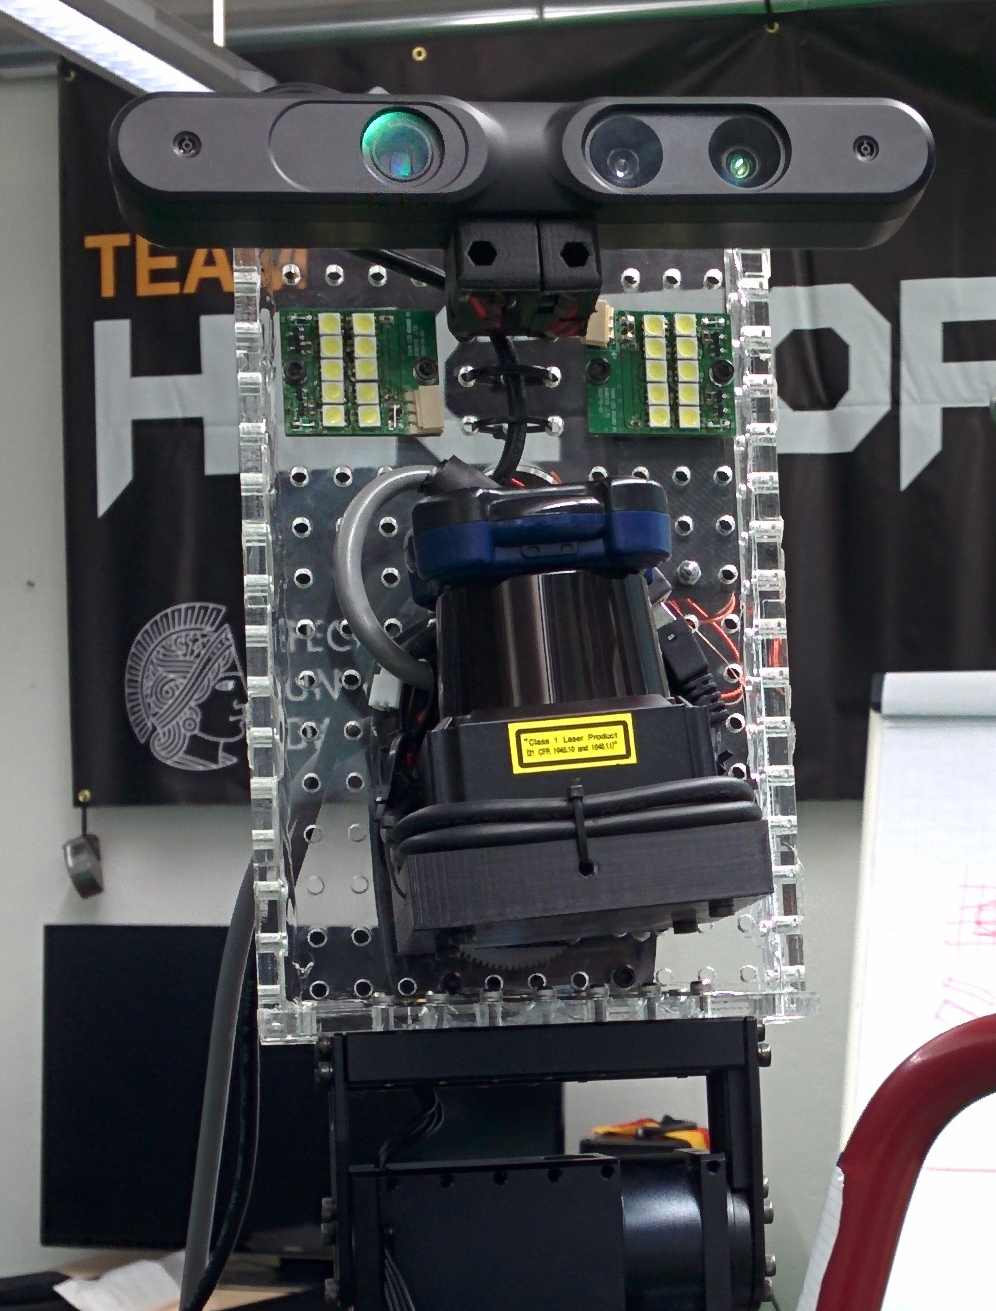
\includegraphics[width=3.5cm]{images/kopf}
	\caption{THOR-OPs Sensorkopf} 
      \end{figure}
  
    \end{columns}


\end{frame}


\subsection*{Motivation für Sensorfusions-Framework}
\begin{frame}[t]
    \frametitle{Motivation für Sensorfusions-Framework}

    \begin{itemize}
      \item Stärken von Sensoren kombinieren
      \item Schwächen ausmerzen
      \item Bestätigung der Daten von anderen Sensoren
      \item Verbesserung der Zuverlässigkeit der Umgebungsmodellierung
      \item Möglichkeiten eines guten (3D-) Weltmodells
      \begin{itemize}
	\item Fußschrittplanung
	\item Kollisionsvermeidung
	\item Pfadplanung
	\item Manipulationsaufgaben
	%\item Immersion bei Fernsteuerung
      \end{itemize}

\end{itemize}
\end{frame}


\subsection*{Anforderungen für Sensorfusions-Framework}






\begin{frame}[t]
  \frametitle{Anforderungen für Sensorfusions-Framework}
      
  \begin{itemize}
      \item Unterstützung beliebig vieler Sensoren
      \item Modellierung der Roboter-Umgebung 
      \item "`Echtzeit"'-Aktualisierungen
      \item Generierung von verschiedenen Umgebungsrepräsentationen
%       \begin{itemize}
% 	\item Höhenkarte
% 	\item Oberflächennormalen-Schätzung
%       \end{itemize}

      \item Effiziente CPU- und Speichernutzung
      \item Anwendbar für verschiedene Roboter und Sensorkonfigurationen
      \item ROS-Integration
  \end{itemize}

     

\end{frame}    





  \section{Grundlagen} 

\subsection*{Truncated Signed Distance Field - TSDF}

\begin{frame}[t]
    \frametitle{Grundlagen: Truncated Signed Distance Fields - TSDF}

    \begin{columns}[t]
      \column[]{7cm}
      
      \begin{itemize}
       \item Signed distance function $\Phi: \mathbf{R}^3 \to \mathbf{R}$ \\ $\rightarrow$ Distanz von Voxel zu Objektoberfläche
       \item $\Phi$ überschreitet Schwellwert $\tau$ \\ $\rightarrow$ Wird abgeschnitten 
      \end{itemize}
      \begin{equation*}
	      \Phi_{\tau}(\mathbf{x}) =
	      \begin{cases}
		      \Phi(\mathbf{x}) &  \text{wenn } | \Phi(\mathbf{x})| < \tau \\
		      \text{undefiniert} & \text{sonst}
	      \end{cases}
      \end{equation*}    
      \begin{itemize}
       \item  Gewicht vom Voxel: Gewissheit der SDF-Schätzung
       \item  Oberflächenverlauf implizit beschrieben
       \item Ermöglicht hochqualitative Oberflächen
      \end{itemize}
     

      \column{5cm}
      
    \begin{figure}[t]
      %\centering
      \vspace{-1cm}
      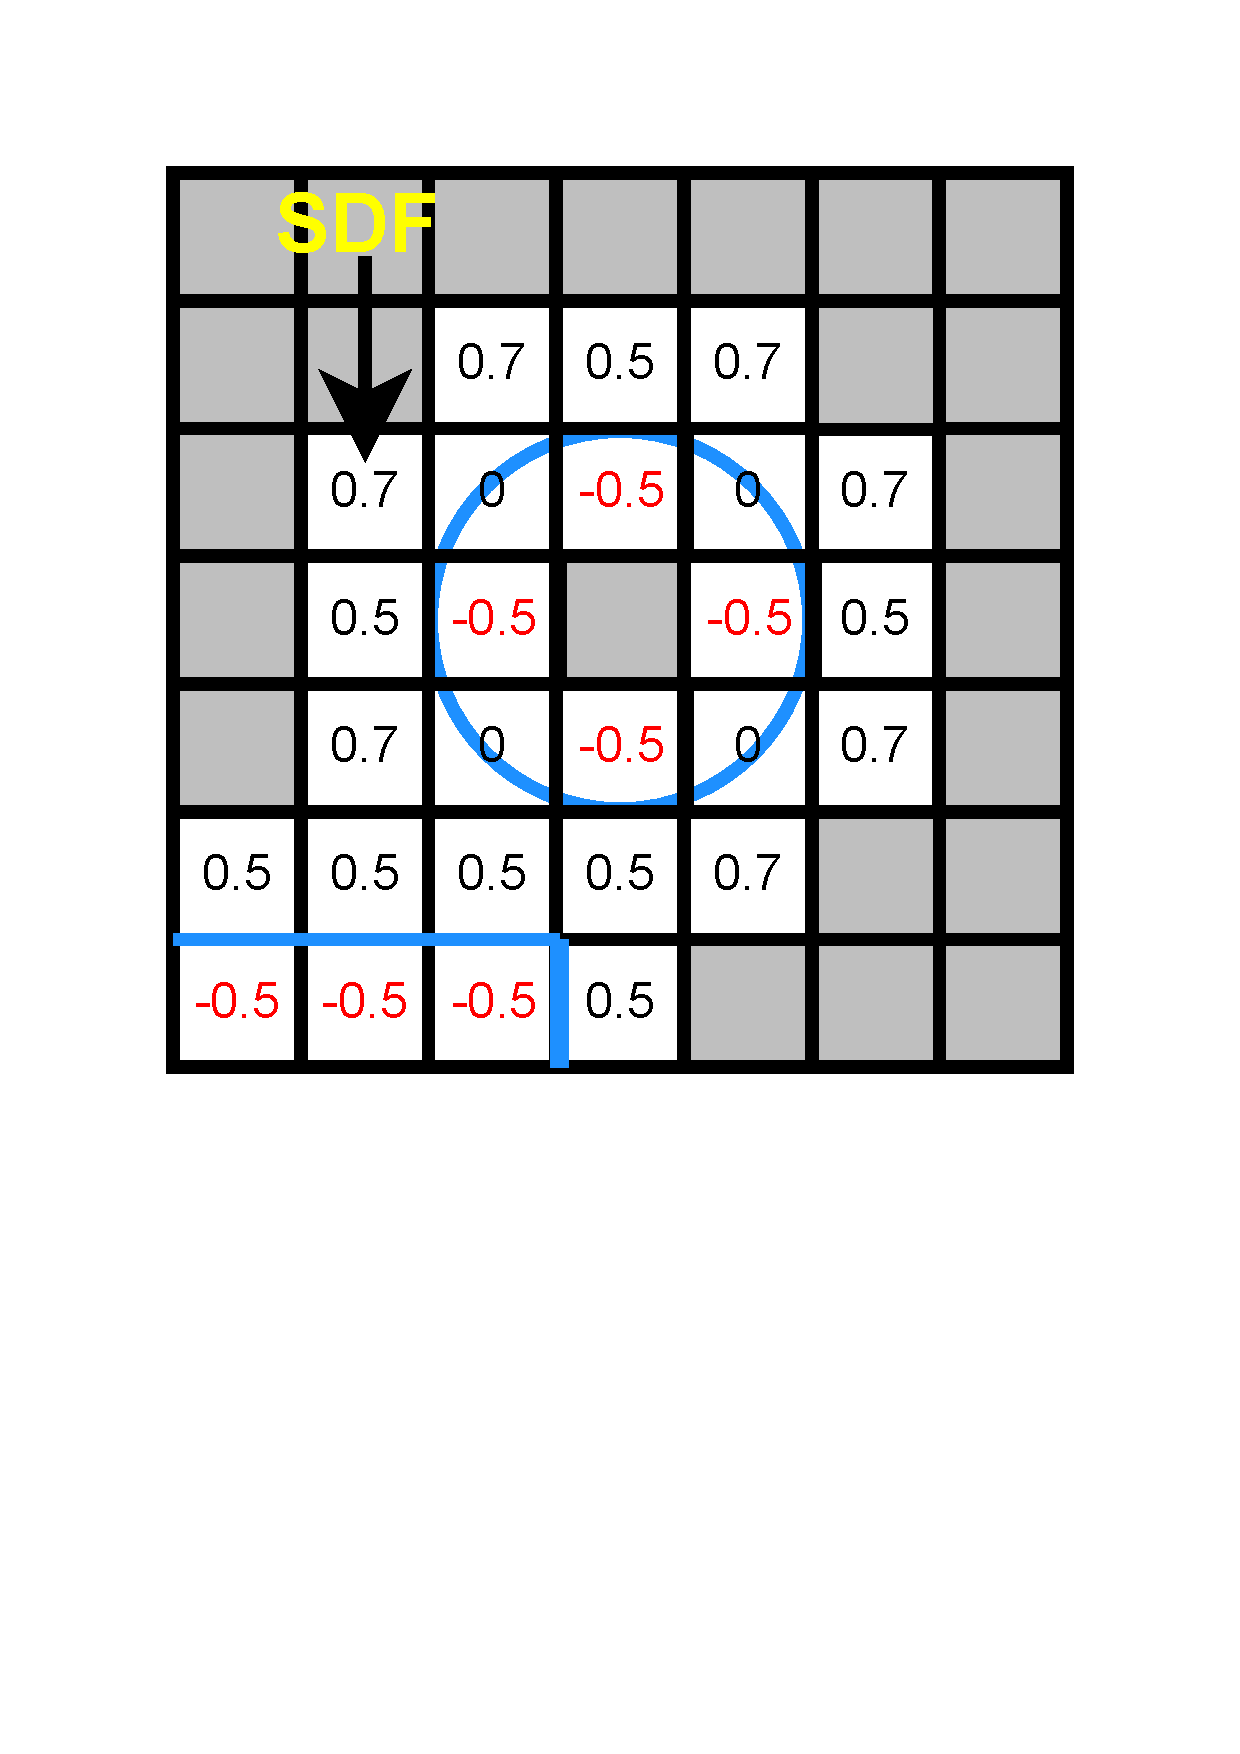
\includegraphics[trim=0 300 0 0, clip, width= \textwidth]{diagrams/tsdf.pdf}
      \caption{2D-TSDF-Voxelgitter} 

    \end{figure}
  
    \end{columns}
    \end{frame}

    \subsection*{Spatially-hashed TSDF}
    
    \begin{frame}[t]
    \frametitle{Grundlagen: Spatially-hashed TSDF}

    \begin{columns}[t]
      \column[]{7cm}
      
      \begin{itemize}
       \item TSDF in Voxelgitter: Sehr speicher- und rechenaufwändig \\ $\rightarrow$ spatially-hashed TSDF
       \item Ausnutzung dünnbesetzter Struktur
       \item Aufteilung der Szene in Voxelblöcke%, die mit Hashtabelle verwaltet  werden
       \item Nur Blöcke mit gültigen TSDF-Daten werden gespeichert
       \item Zugriff auf Voxel bei gegebener Weltposition: $\mathcal O(1)$
      \end{itemize}
     

      \column{5cm}
      
       \begin{figure}[h]
 	\centering
 	    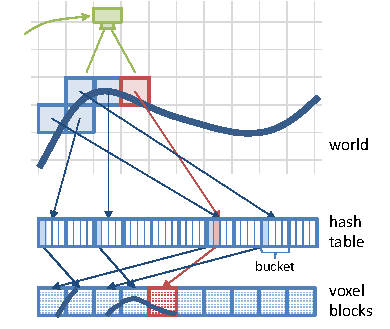
\includegraphics[width=\textwidth]{images/voxel_hashing.pdf}
 	\caption{Aufteilung der Szene in gehashte Voxelblöcke [1]} 
       \end{figure}
  
    \end{columns}
    \end{frame}
  \section{Stand der Forschung} 


\subsection*{Continuous Humanoid Locomotion over Uneven Terrain using Stereo Fusion}

    \begin{frame}[t]
    \frametitle{Stand der Forschung: Continuous Humanoid Locomotion over Uneven Terrain using Stereo Fusion}

    \begin{columns}[t]
      \column[]{6cm}
      
      \begin{itemize}
      \item Team MIT's Ansatz für Fortbewegung auf unebenem Gelände anlässlich DRC Finale
      \item Basiert auf Kintinous
      \begin{itemize}
       \item 3D-TSDF-Struktur für RGB-D Sensorfusion
       \item CUDA-Beschleunigung für Echtzeit-Anwendung
%        \item Verschiebendes Voxelgitter auf GPU ermöglicht größere Szenen 
      \end{itemize}

      \item Anpassung von Kintinous für Stereo Kamera (ATLAS Roboter)
%       \item 3D-Karte genutzt für Fußschrittplanung und Kollisionsvermeidung

     \end{itemize}
     

      \column{6cm}
      
       \begin{figure}[h]
 	\centering
%  	    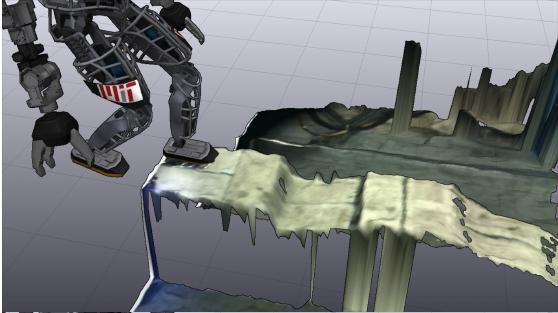
\includegraphics[width=\textwidth]{images/mit_locomotion}
	  \movie[width = 6cm, height = 3.5cm,
                 autostart,loop, poster] 
      {}{video/mit.m4v}
 	\caption{Laufen basierend auf Kintinous [2]} 
       \end{figure}
  
    \end{columns}
    \end{frame}

    
    \begin{frame}[t]
    \frametitle{Stand der Forschung: Continuous Humanoid Locomotion over Uneven Terrain using Stereo Fusion}

    \begin{columns}[t]
      \column[]{6cm}
      \vspace{-0.5cm}
      \begin{exampleblock}{Vorteile}
	  \begin{itemize}
	    \item Performant durch GPU-Beschleunigung
	  \end{itemize} 
	\end{exampleblock}
	
	\begin{alertblock}{Nachteile}
	 \begin{itemize}
	\item GPU-Nutzung schränkt mögliche Anwendungsfälle ein
	\item Gebiete außerhalb des Kamera-Blickfeldes werden tesseliert 
	\begin{itemize}
	\item Löschen der TSDF-Daten
	\end{itemize}
	\item Unterstützung von nur einem Sensor

      \end{itemize}
	\end{alertblock}
     

      \column{6cm}
      
       \begin{figure}[h]
 	\centering
%  	    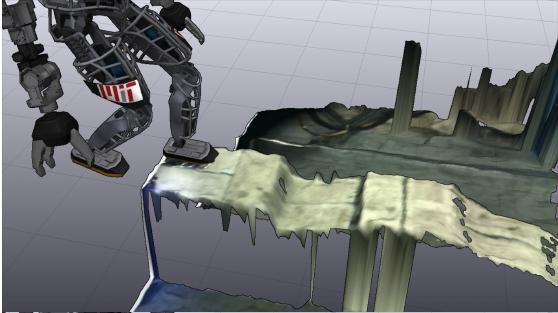
\includegraphics[width=\textwidth]{images/mit_locomotion}
	  \movie[width = 6cm, height = 3.5cm,
                 autostart,loop, poster] 
      {}{video/mit.m4v}
 	\caption{Laufen basierend auf Kintinous [2]} 
       \end{figure}
  
    \end{columns}
    \end{frame}

 \subsection*{Robot-Centric Elevation Mapping}
 
    \begin{frame}[t]
    \frametitle{Stand der Forschung: Robot-Centric Elevation Mapping}

    \begin{columns}[t]
      \column[]{6cm}
      
      \begin{itemize}
      \item  ETH Zürich, 2014
      \item  Erstellung von Höhenkarten (2,5D) für mobile Roboter 
      \item  Kalman-Filter für Fusion der Höhenschätzungen inklusive Abschätzung von Unsicherheit
      \item  ROS-Integration 
      \item  CPU-basiert


     \end{itemize}
     

      \column{6cm}
      
       \begin{figure}[h]
 	\centering
%  	    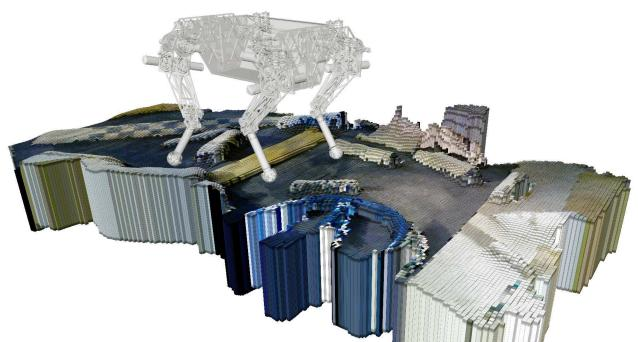
\includegraphics[width=\textwidth]{images/eth_elevation_mapping}
 	  \movie[width = 6cm, height = 3.4cm,
                 autostart,loop, poster] 
{}{video/eth.mp4}
 	\caption{Erstellung der Höhenkarte [3]} 
       \end{figure}
  
    \end{columns}
    \end{frame}

    \begin{frame}[t]
    \frametitle{Stand der Forschung: Robot-Centric Elevation Mapping}
      
      \begin{columns}[t]
      \column[]{6cm}
      \vspace{-0.5cm}
        
	\begin{exampleblock}{Vorteile}
	  \begin{itemize}
	    \item Anwendung auf vielen Robotersystemen möglich durch CPU-Nutzung
	    \item 2,5D Darstellung
	    \begin{itemize}
	    \item Hohe Aktualisierungsrate
	    \item Geringer Speicherverbrauch
	    \end{itemize} 

	  \end{itemize} 
	\end{exampleblock}
	
	\begin{alertblock}{Nachteile}
	\begin{itemize}
	  \item Nur ein Distanzsensor unterstützt
	  \item Form der Weltdarstellung nicht immer geeignet
	\end{itemize}

	\end{alertblock}
     
     \column{6cm}
      
       \begin{figure}[h]
 	\centering
 	    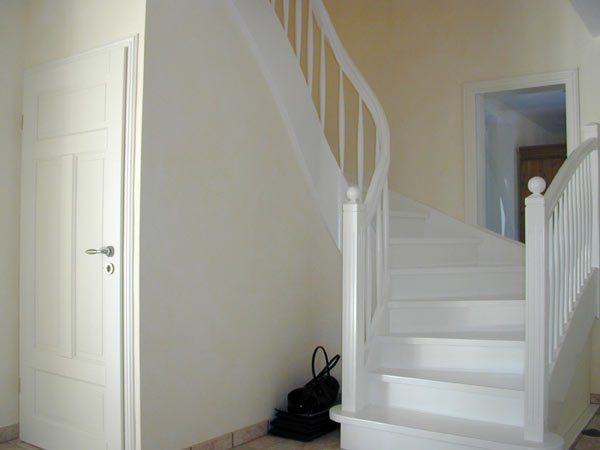
\includegraphics[width=\textwidth]{images/raum_unter_treppe}
 	\caption{Raum unter Treppe   [4]} 
       \end{figure}
  
    \end{columns}
     
    \end{frame}
    
    
    
\subsection*{Obviously}


    \begin{frame}[t]
    \frametitle{Stand der Forschung: Obviously}
      
      \begin{columns}[t]
      \column[]{7cm}
      
      \begin{itemize}
      \item TH Nürnberg, 2014
      \item Multisensor-Fusions-Framework für Umgebungsmodellierung
      \item Echtzeit-Anwendung für mobile Roboter
      \item CPU-gestütztes TSDF
     % \item Hinzufügen von neuen Sensoren: Implementierung des Sensormodell-Interfaces
      \item Keine ROS-Integration 
      
      
     \end{itemize}
     
     \column{5cm}
      
       \begin{figure}[h]
       \vspace{-0.5cm}
 	\centering
 	    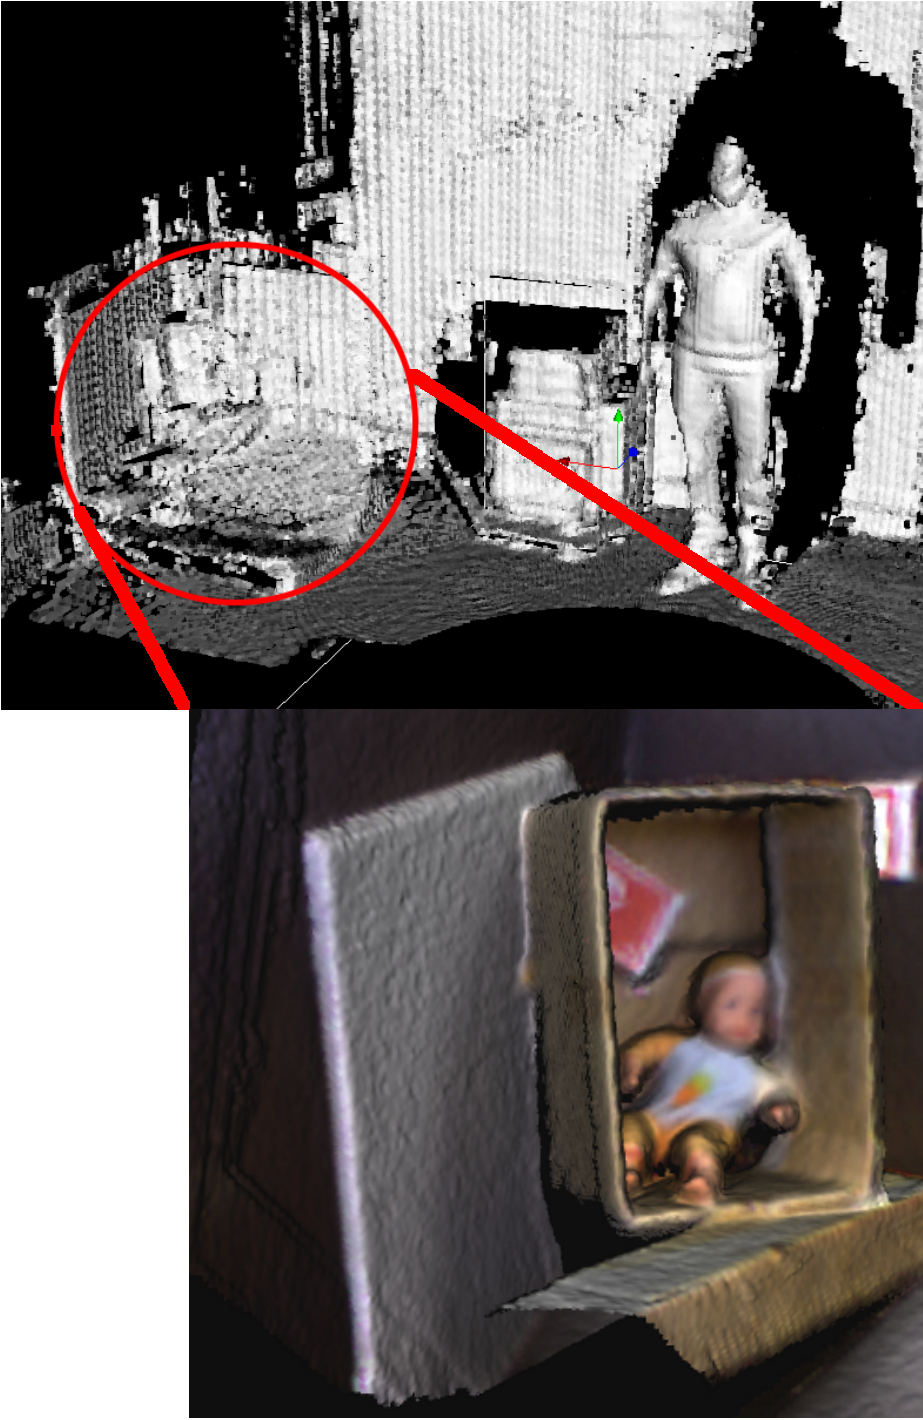
\includegraphics[width=0.65\textwidth]{images/obviosly_concat}
 	\caption{Einsatz von Obviously [5]} 
       \end{figure}
  
    \end{columns}
     
    \end{frame}
    
    \begin{frame}[t]
    \frametitle{Stand der Forschung: Obviously}
      
      \begin{columns}[t]
      \column[]{7cm}
      \vspace{-0.5cm}
        \begin{exampleblock}{Vorteile}
	  \begin{itemize}
	    \item Mehrere Sensoren fusionierbar
	    \item Verschiedene Repräsentationen für Weltmodell verfügbar
	  \end{itemize} 
	\end{exampleblock}
	
	\begin{alertblock}{Nachteile}
	        \begin{itemize}
	\item Voxelgitter für TSDF-Daten
	\item Leere Voxelblöcke werden gespeichert und aktualisiert\\
	$\rightarrow$ Unnötige Verwendung von Speicher und Rechenzeit 
	\item Hinzufügen von neuen Sensoren aufwendig 
      \end{itemize} 
	\end{alertblock}
     
     \column{5cm}
      
       \begin{figure}[h]
       \vspace{-0.5cm}
 	\centering
 	    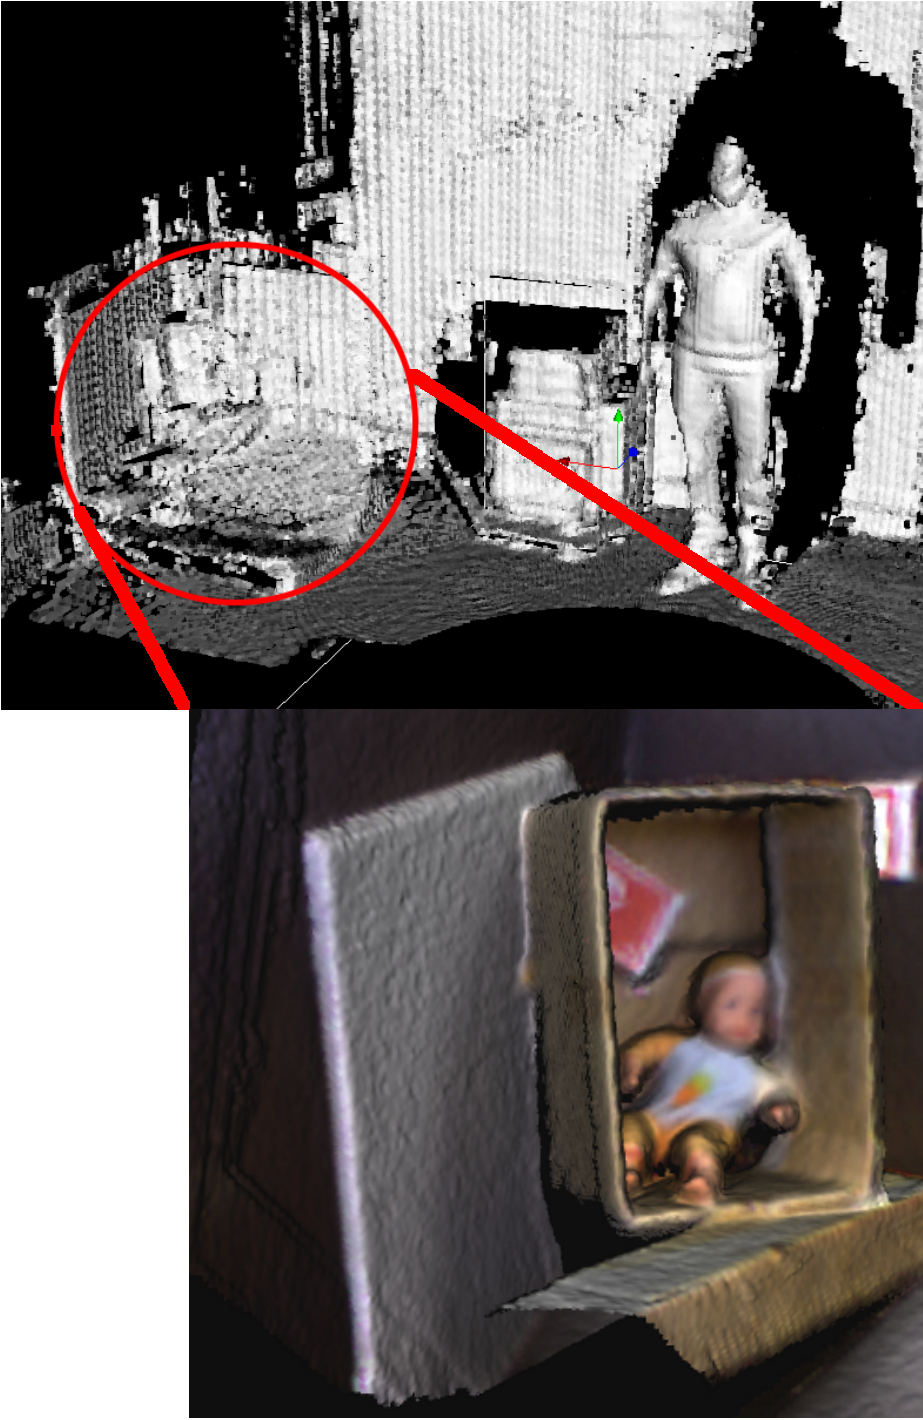
\includegraphics[width=0.65\textwidth]{images/obviosly_concat}
 	\caption{Einsatz von Obviously [5]} 
       \end{figure}
  
    \end{columns}
     
    \end{frame}
    
\subsection*{Vigir Terrain Classifier}

\begin{frame}[t]
  \frametitle{Stand der Forschung: Vigir Terrain Classifier}
      
     \begin{columns}[t]
      \column[]{6cm}
     
      \begin{itemize}
	\item Akkumulation von Laserscans
	\item Octree mit fester Knotengröße
	\item Erzeugt Höhenkarte und Oberflächennormalen-Schätzung
	\item Nur Daten im Bereich um neusten Laserscan geupdated
      \end{itemize} 
     
     \column{6cm}
     

       \begin{figure}[h]
       \vspace{-0.5cm}
	  \movie[width = 6cm, height = 3.5cm,
                 autostart,loop, poster] 
{}{video/drop.avi}
 	\caption{Laufen mit Vigir Terrain Classifier [6]} 
       \end{figure}

  
    \end{columns}  
      
\end{frame}


\begin{frame}[t]
  \frametitle{Stand der Forschung: Vigir Terrain Classifier}
      
     \begin{columns}[t]
      \column[]{6cm}
      
       \begin{exampleblock}{Vorteile}
	  \begin{itemize}
	  %\item Nur eine Datenschicht
	    \item Hohe Aktualisierungsraten möglich
	  \end{itemize} 
	\end{exampleblock}
	  
	\begin{alertblock}{Nachteile}
	  \begin{itemize}
	      %\item Nur eine Datenschicht
		\item Keine Abschätzung der Sicherheit von Höhenmessungen
		\item Dynamische Objekte "`zerstören"' Umgebungsmodellierung
		\item Nur ein Sensor wird unterstützt
	      \end{itemize} 
	    \end{alertblock}
	    
     \column{6cm}

       \begin{figure}[h]
       \vspace{-0.5cm}
	  \movie[width = 6cm, height = 3.5cm,
                 autostart,loop, poster] 
{}{video/vigir_terrain.mp4}
 	\caption{Laufen mit Vigir Terrain Classifier [6]} 
       \end{figure}

  
    \end{columns}  
      
\end{frame}

 \subsection*{CHISEL}
 
\begin{frame}[t]
  \frametitle{Stand der Forschung: CHISEL}
  
  \begin{columns}[t]
      \column[]{6cm}
      
      \begin{itemize}
      \item CMU, 2015
      \item Bibliothek für 3D-Rekonstruktion großer Volumen in Echtzeit
      \item Ursprünglich für mobile Geräte mit Tiefensensor
      \item Spatially-hashed TSDF nur mit CPU
     % \begin{itemize}
       %\item Experiment: 93\% der Voxel leer
       %\item Wieso speichern und aktualisieren?
      %\end{itemize}

      \item Beachtung von Sensor-Messfehlern
     \end{itemize}
     
     \column{6cm}
      
      \begin{figure}[h]
%  	\centering
% 	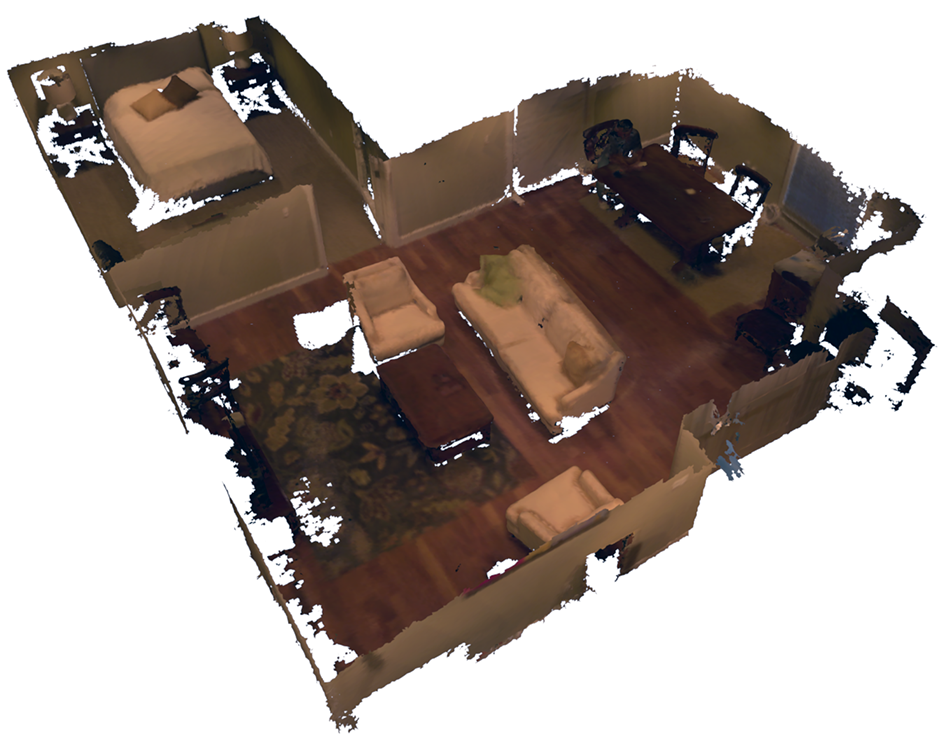
\includegraphics[width=0.65\textwidth]{images/chisel}
	  \movie[width = 6cm, height = 3.5cm,
                 autostart,loop, poster] 
{}{video/chisel_trim.m4v}
 	\caption{Szene rekonstruiert durch CHISEL [7]} 
      \end{figure}
  
    \end{columns}
\end{frame}

\begin{frame}[t]
  \frametitle{Stand der Forschung: CHISEL}
  
  \begin{columns}[t]
      \column[]{6cm}
      
  \begin{exampleblock}{Vorteile}
  \begin{itemize}
    \item ROS-Integration
    \item Sehr leistungsfähige Bibliothek
    \item TSDF-Daten bleiben erhalten
  \end{itemize} 
  \end{exampleblock}
  
  \begin{alertblock}{Nachteile}
    \begin{itemize}
      \item Support für nur einen Distanzsensor
      \item Keine Posenschätzung vorhanden \\ $\rightarrow$ externe Posenschätzung benötigt
    \end{itemize} 
  \end{alertblock}
     
     \column{6cm}
      
      \begin{figure}[h]
%  	\centering
% 	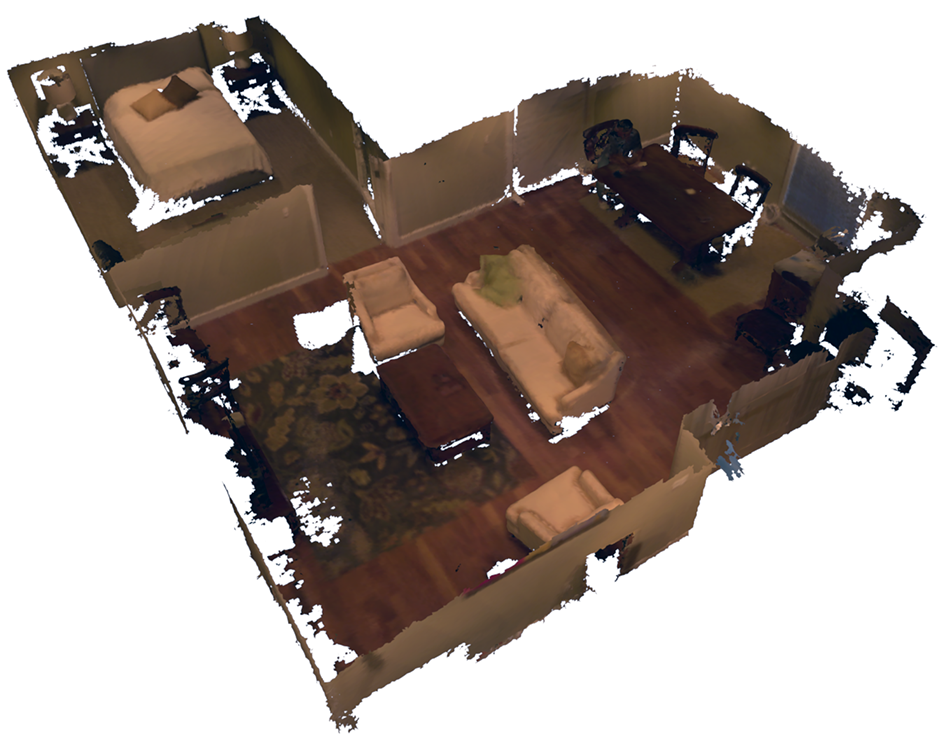
\includegraphics[width=0.65\textwidth]{images/chisel}
\movie[start=35s,width = 5.5cm, height = 3.5cm,
                 autostart,repeat,poster] 
{}{video/chisel_trim.m4v}
 	\caption{Szene rekonstruiert durch CHISEL [7]} 
      \end{figure}
  
    \end{columns}
\end{frame}

 
  \section{Konzept} 

\begin{frame}[c]
    \frametitle{Konzept: Framework-Klassen}
      
    \begin{figure}[t]
      %\centering
      \vspace{-0.8cm}
      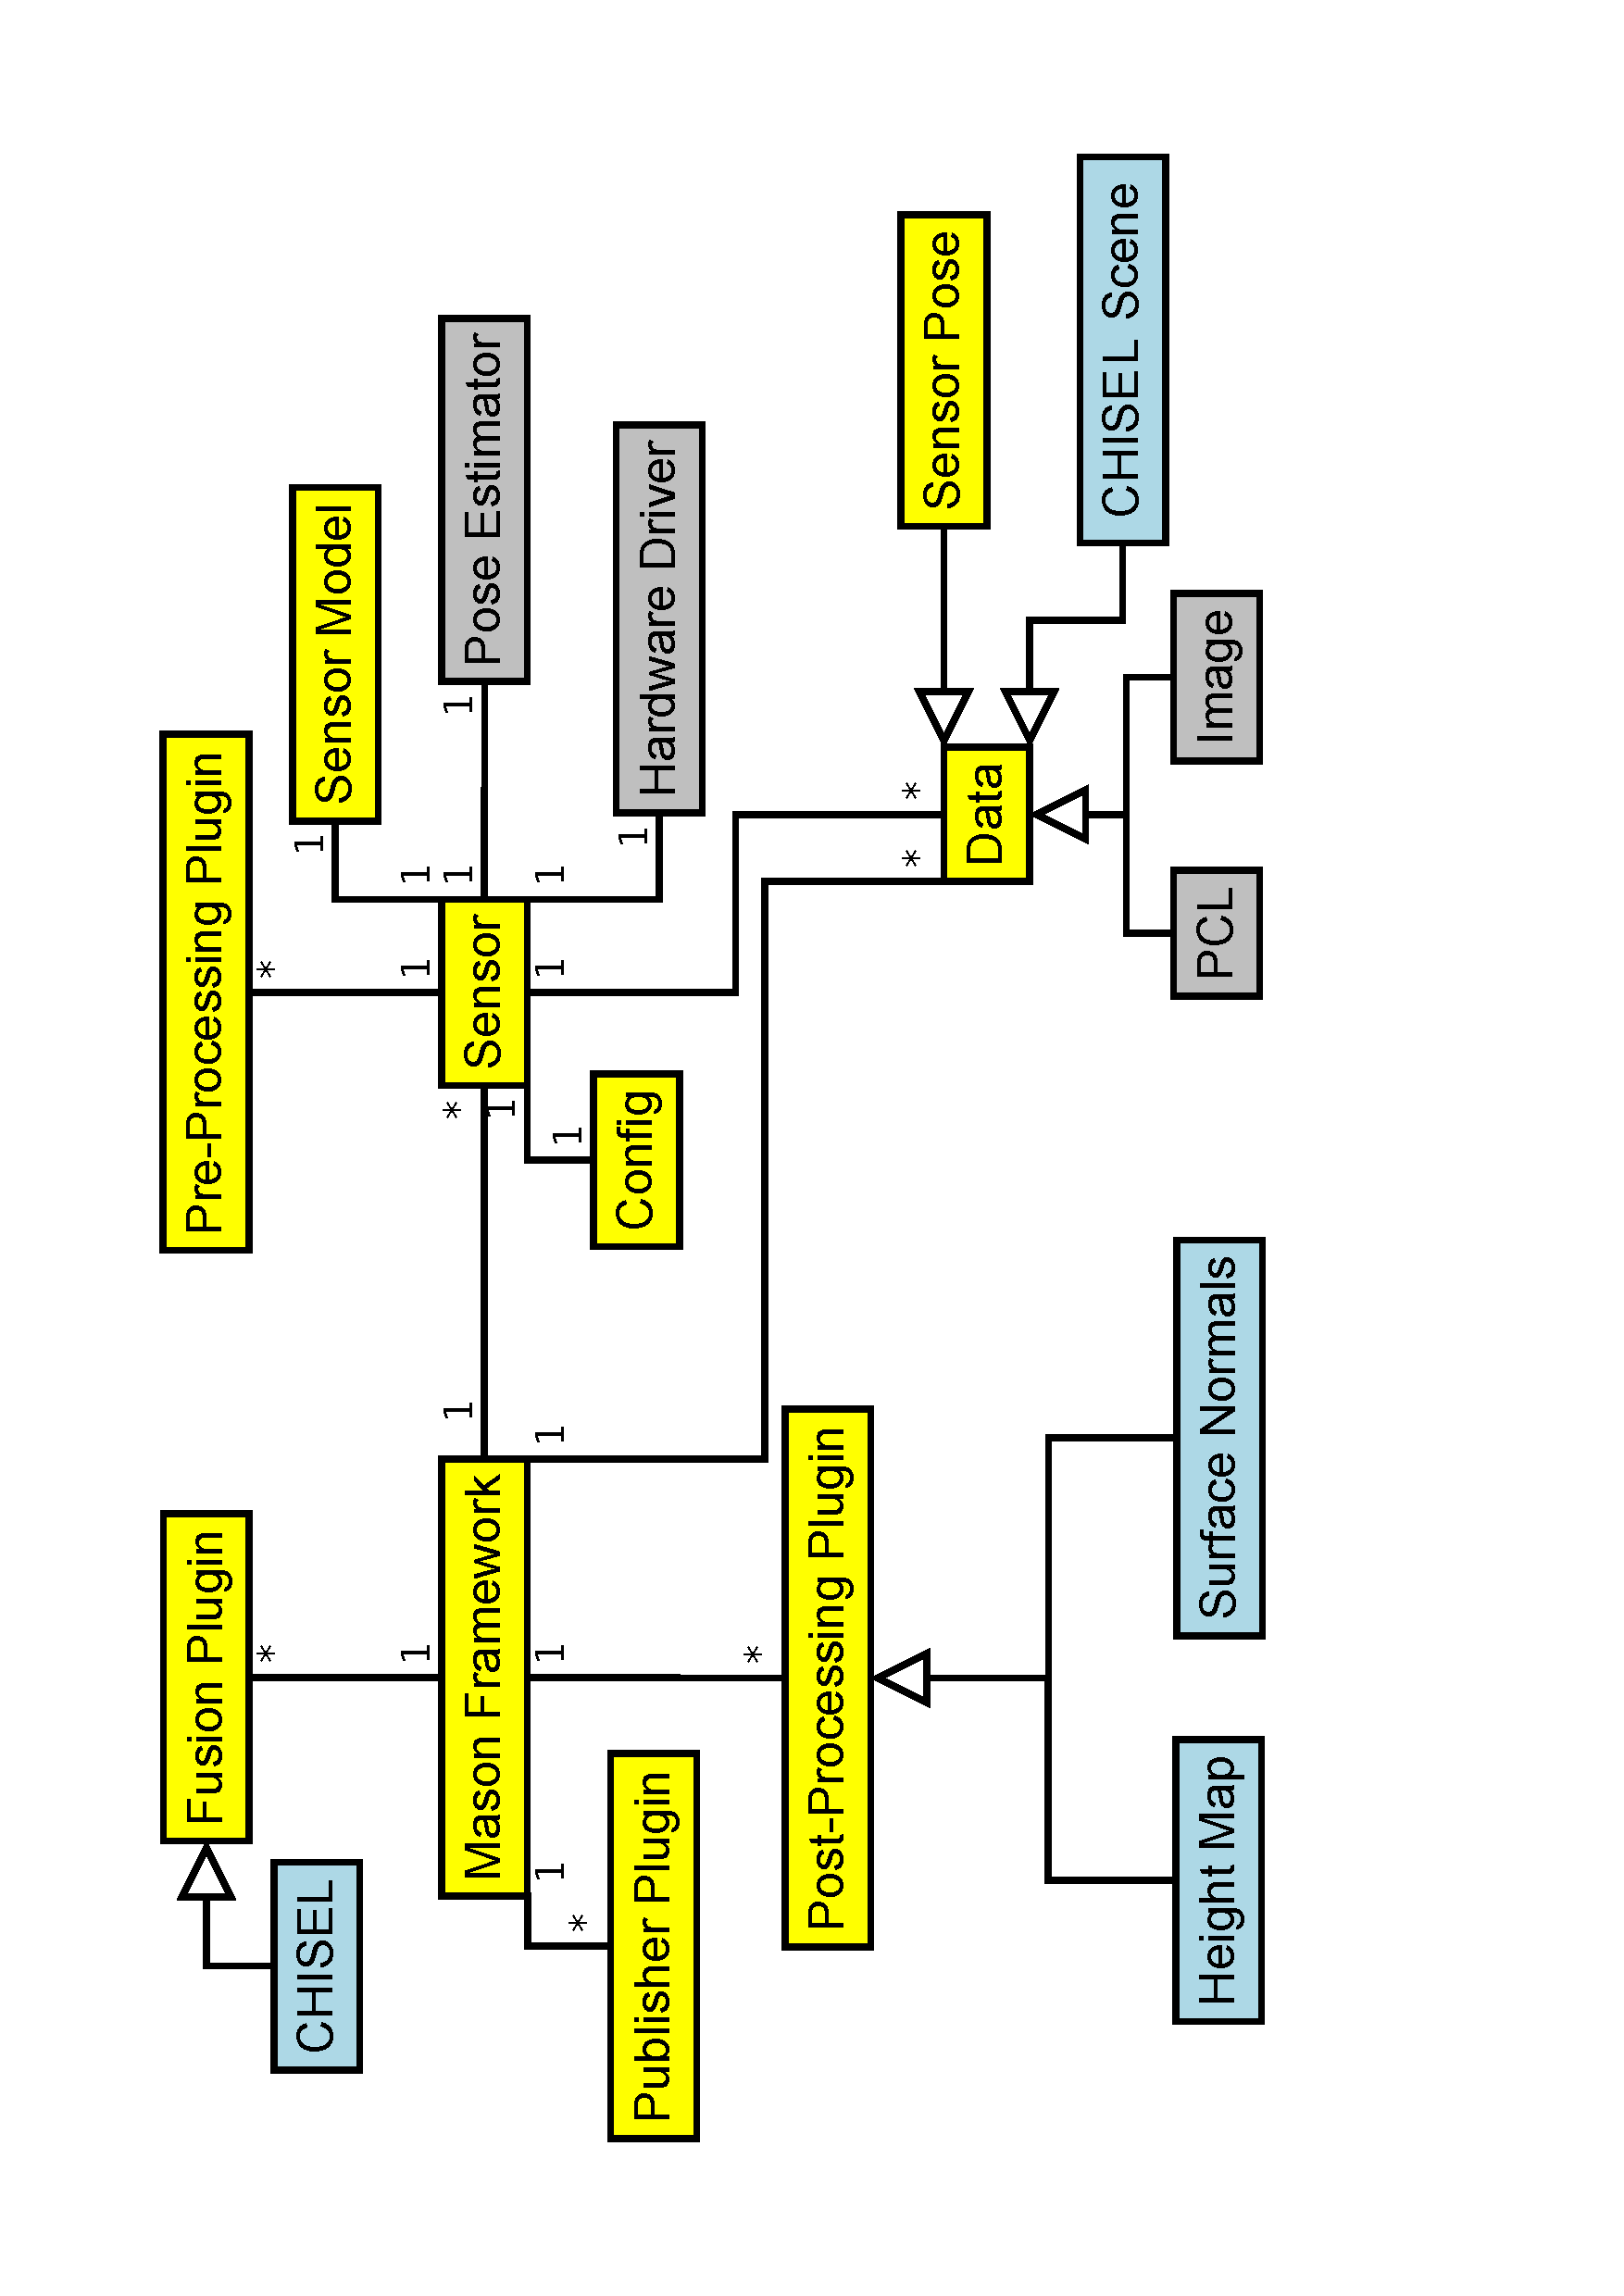
\includegraphics[angle=270,origin=c, width= \textwidth]{diagrams/framework_concept.pdf}
      \label{fig:preprocessing_phase}
    \end{figure}
 
    \end{frame}


\begin{frame}[c]
    \frametitle{Konzept: Pipeline}
      
    \begin{figure}[t]
      %\centering
      \vspace{-0.8cm}
      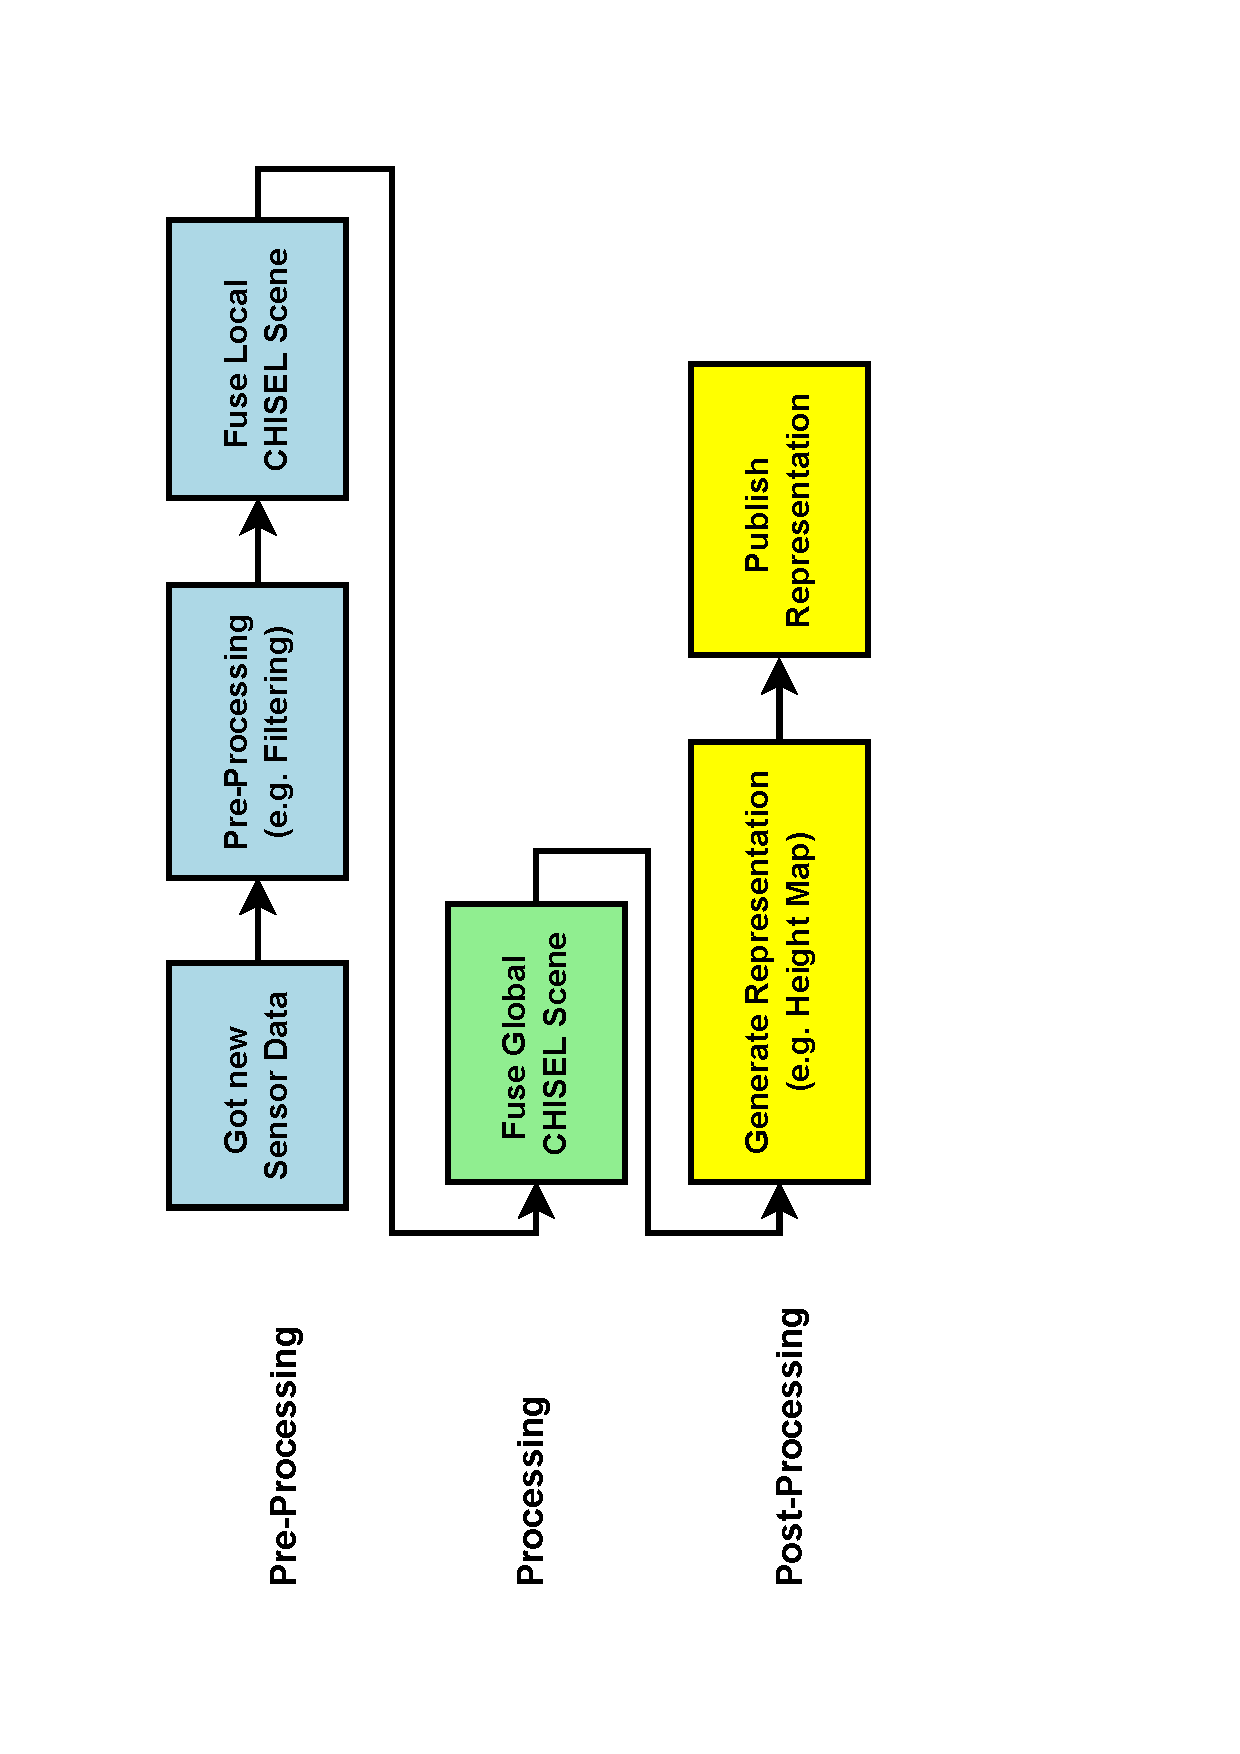
\includegraphics[angle=270,origin=c, width= \textwidth]{diagrams/pipeline.pdf}
      \label{fig:preprocessing_phase}
    \end{figure}
 
\end{frame}

\section{Aktueller Stand und Aussicht}

    \begin{frame}[t]
    \frametitle{Aktueller Stand und Aussicht}
      
      \begin{columns}[t]
      \column{5cm}
     \begin{itemize}
     \item Fusion von verschiedenen Sensoren möglich \\ $\rightarrow$ CHISEL Fusion-Plugin
      \begin{itemize}
	\item  Beliebige Voxelblock-Größen und Auflösungen
	\item  Auch mit Farbinformationen
	\item  Oberflächennormalen-Schätzung 
      \end{itemize}
     \item Tiefenbilder und Pointclouds integrierbar

      \end{itemize}
     
     \column{7cm}
      
       \begin{figure}[h]
 	\centering
 	    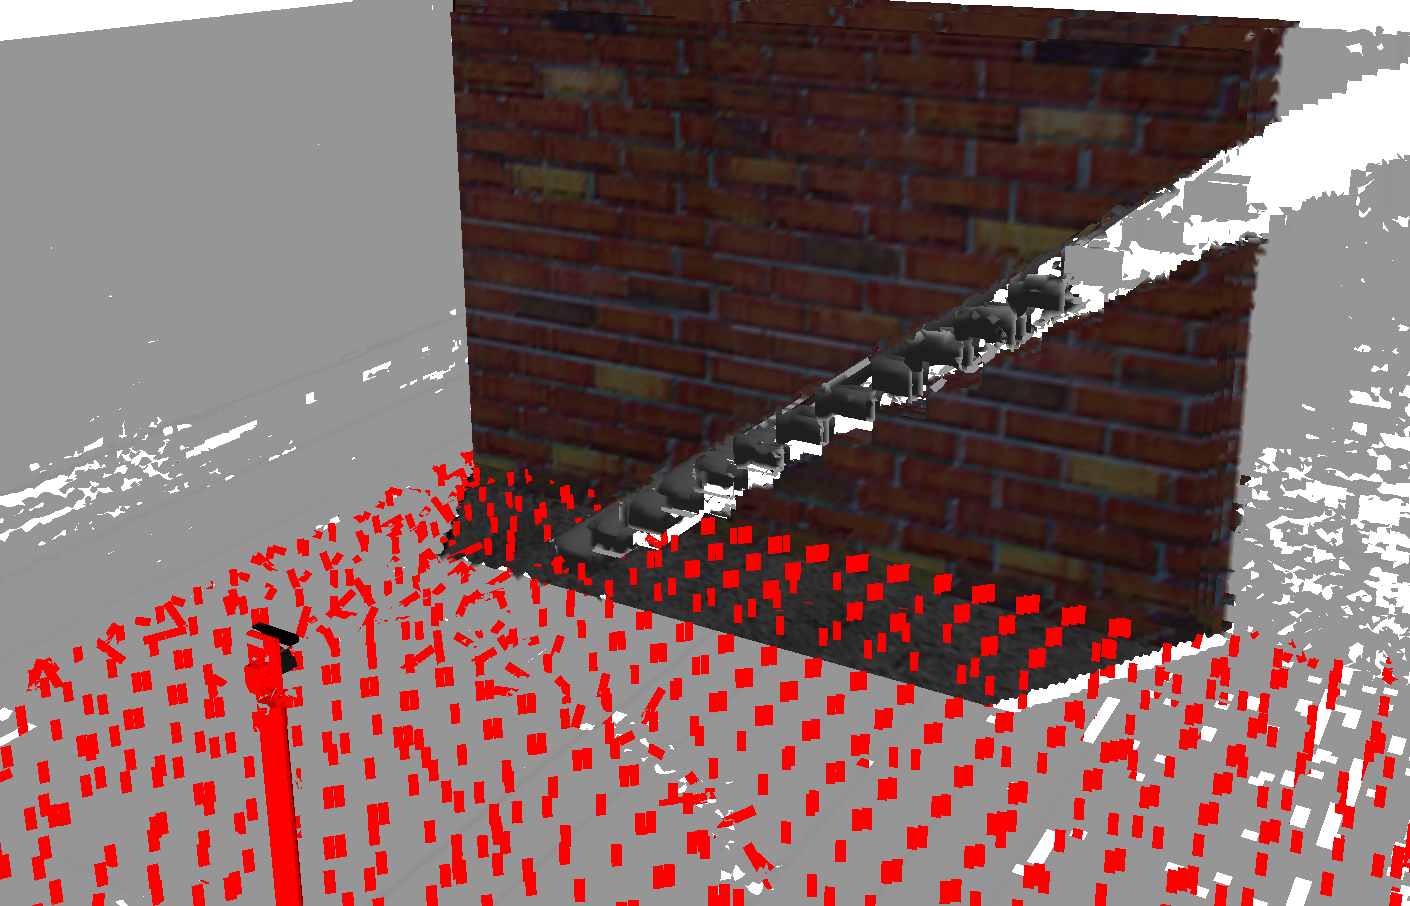
\includegraphics[width=0.9\textwidth]{images/mason_trim}
 	\caption{Fusion von RGB-D- und Laserscanner-Daten} 
       \end{figure}
  
    \end{columns}
     
    \end{frame}

\begin{frame}[c]
    \frametitle{Zusammenfassung und Aussicht}
      

    \begin{block}{Zusammenfassung}
      \begin{itemize}
       \item CHISEL als performante Basis für Multisensor-Fusions-Framework
       \item Spatially-hashed TSDF 
       \item Erstellung von verschiedenen Repräsentationen aus Weltmodell
      \end{itemize}

    \end{block}


      \begin{block}{Aussicht}
	\begin{itemize}
	  \item Implementierung vom Framework
	  \begin{itemize}
	   \item Übertragen vom aktuellen Stand in Plugins
	   \item Interface vom Framework zu CHISEL
	   %\item Fehler ausbessern

	  \end{itemize}

	  \item Evaluation
	  \begin{itemize}
	   \item Leistung
	   \item Zusammenspiel verschiedener Sensorkonfigurationen (Gazebo und Roboter)
	   \item Zuverlässigkeit
	  \end{itemize}

	\end{itemize} 
      
      \end{block}
    
    

\end{frame}
   

  \section*{Quellen}

\begin{frame}[allowframebreaks]
\frametitle{Referenzen}
\begin{thebibliography}{8}
\bibitem{niessner2013real}[Nie{\ss}ner, 2013]
M. Nie{\ss}ner, M. Zollhöfer, S. Izadi, et al.
\newblock Real-time 3d reconstruction at scale using voxel hashing
\newblock ACM Transactions on Graphics (TOG), 2013.

\bibitem{fallon15humanoids}[Fallon, 2015]
M. Fallon, P. Marion, R. Deits , et al.
\newblock Continuous Humanoid Locomotion Over Uneven Terrain Using Stereo Fusion
\newblock International Conference on Humanoid Robots, 2015.
\newblock Video: \small{\url{https://www.youtube.com/watch?v=_6WQxXH-bB4}}

\bibitem{Fankhauser2014RobotCentricElevationMapping}[Fankhauser, 2014]
P. Fankhauser, M. Bloesch, C. Gehring, et al.
\newblock Robot-Centric Elevation Mapping with Uncertainty Estimates
\newblock International Conference on Climbing and Walking Robots (CLAWAR), 2014.
\newblock Video: \small{\url{https://www.youtube.com/watch?v=I9eP8GrMyNQ}}

\bibitem{niessner2013real}[zuhause.de]
\newblock \small{ \url{http://bilder.zuhause.de/b/56/21/79/18/id_56217918/tid_da/den-raum-unter-der-treppe-nutzen.jpg}}

\bibitem{may2014generalized}[May, 2014]
S. May, P. Koch, R. Koch, et al.
\newblock A Generalized 2D and 3D Multi-Sensor Data Integration Approach based on Signed Distance Functions for Multi-Modal Robotic Mapping
\newblock VMV, 2014.

\bibitem{stumpf}[Stumpf]
A. Stumpf
\newblock Vigir Terrain Classifier

\bibitem{klingensmithchisel}[Klingensmith, 2015]
M. Klingensmith, I. Dryanovski, S. S. Srinivasa, et al.
\newblock Chisel: real time large scale 3d reconstruction onboard a
mobile device using spatially-hashed signed distance fields,
\newblock Robotics Science and Systems, 2015.
\newblock Video: \small{\url{https://vimeo.com/117544631}}


\end{thebibliography}
\end{frame}
  
\end{document}
